\section{Prototypes}\label{sec:prototypes-design}
To get a clear view of how the different pages will look and catch any early potential design problems, we have created prototypes for each of the different pages. 
We will use these to make the implementation of the different pages easier to ensure that we have a consistent design throughout the system. 
The prototypes will not serve as an exact vision of how the pages will look but will instead serve as a guideline to how the page should be set up.
In this section, we will look at some of the more interesting prototypes where we have had to make some design choices.
\begin{figure}[]
    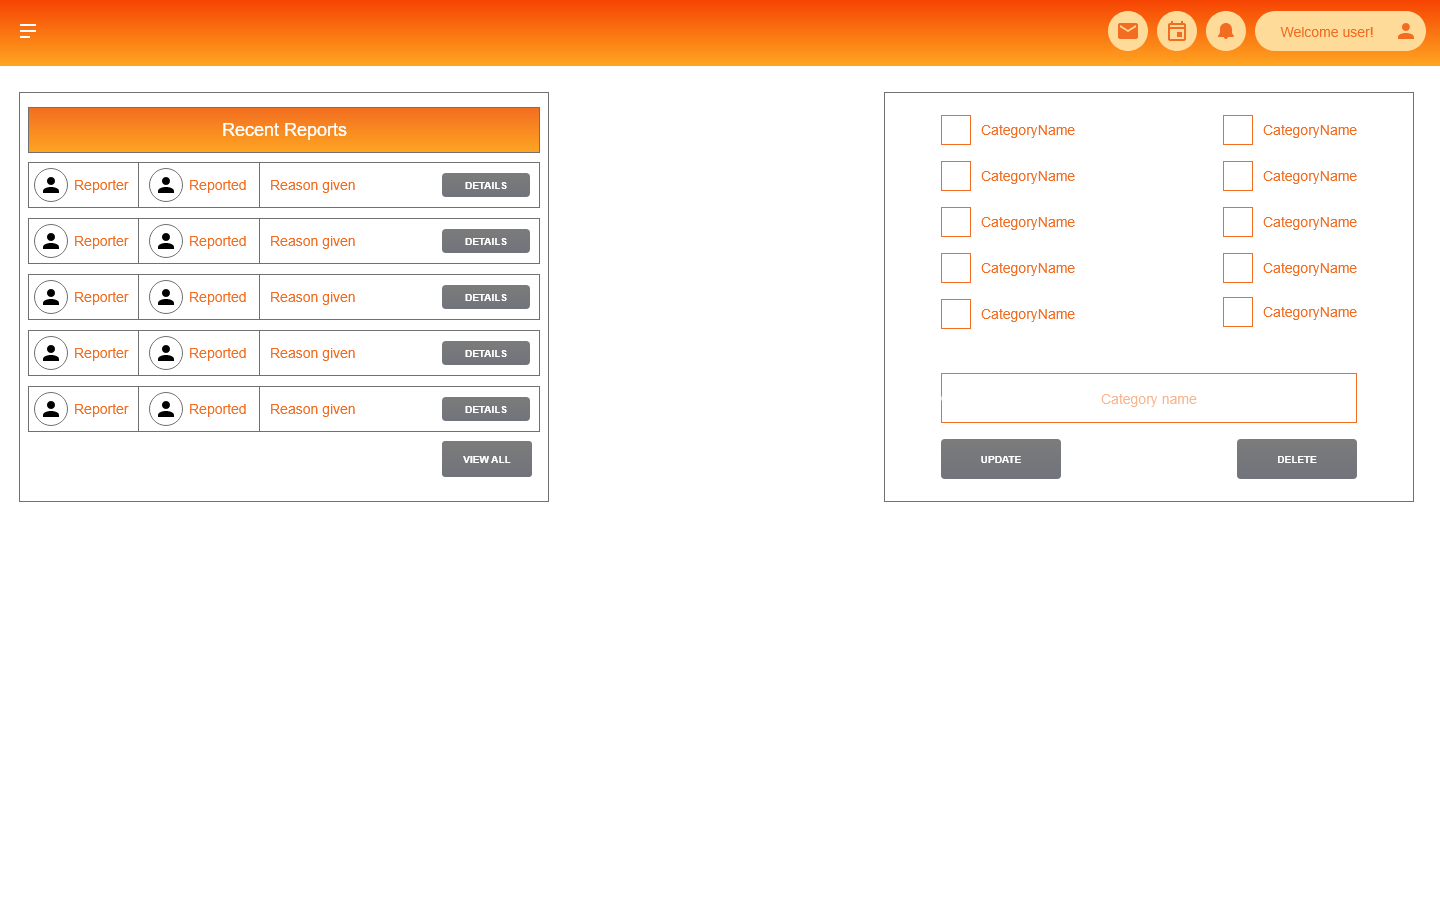
\includegraphics[width=\linewidth]{/prototypes/admin-dashboard.png}
     \caption{Shows the admin dashboard for admins that are logged into the system}
     \label{fig:admin-dashboard}
 \end{figure}
 \noindent
 \\\\
The admin dashboard illustrated in \autoref{fig:admin-dashboard} gives the admin an overview of the recently reported tutors and the different categories. 
The admin needs to see tutor reports since they are the ones that will handle them and decide if a tutor should be banned. 
Admins are also in charge of the different teaching categories, and therefore, they need to have an overview of the current ones and also be able to add new categories.
We also have a top bar that is used on every page for when the user is logged in. It shows a couple of different icons where the user can go to the inbox, the calendar, or the user's own page. 
It will also show notifications for when different events related to the user happen in the system. 
On the far left side of the top bar, we will place a logo, which will lead to the landing page.
\begin{figure}[]
    \centering
   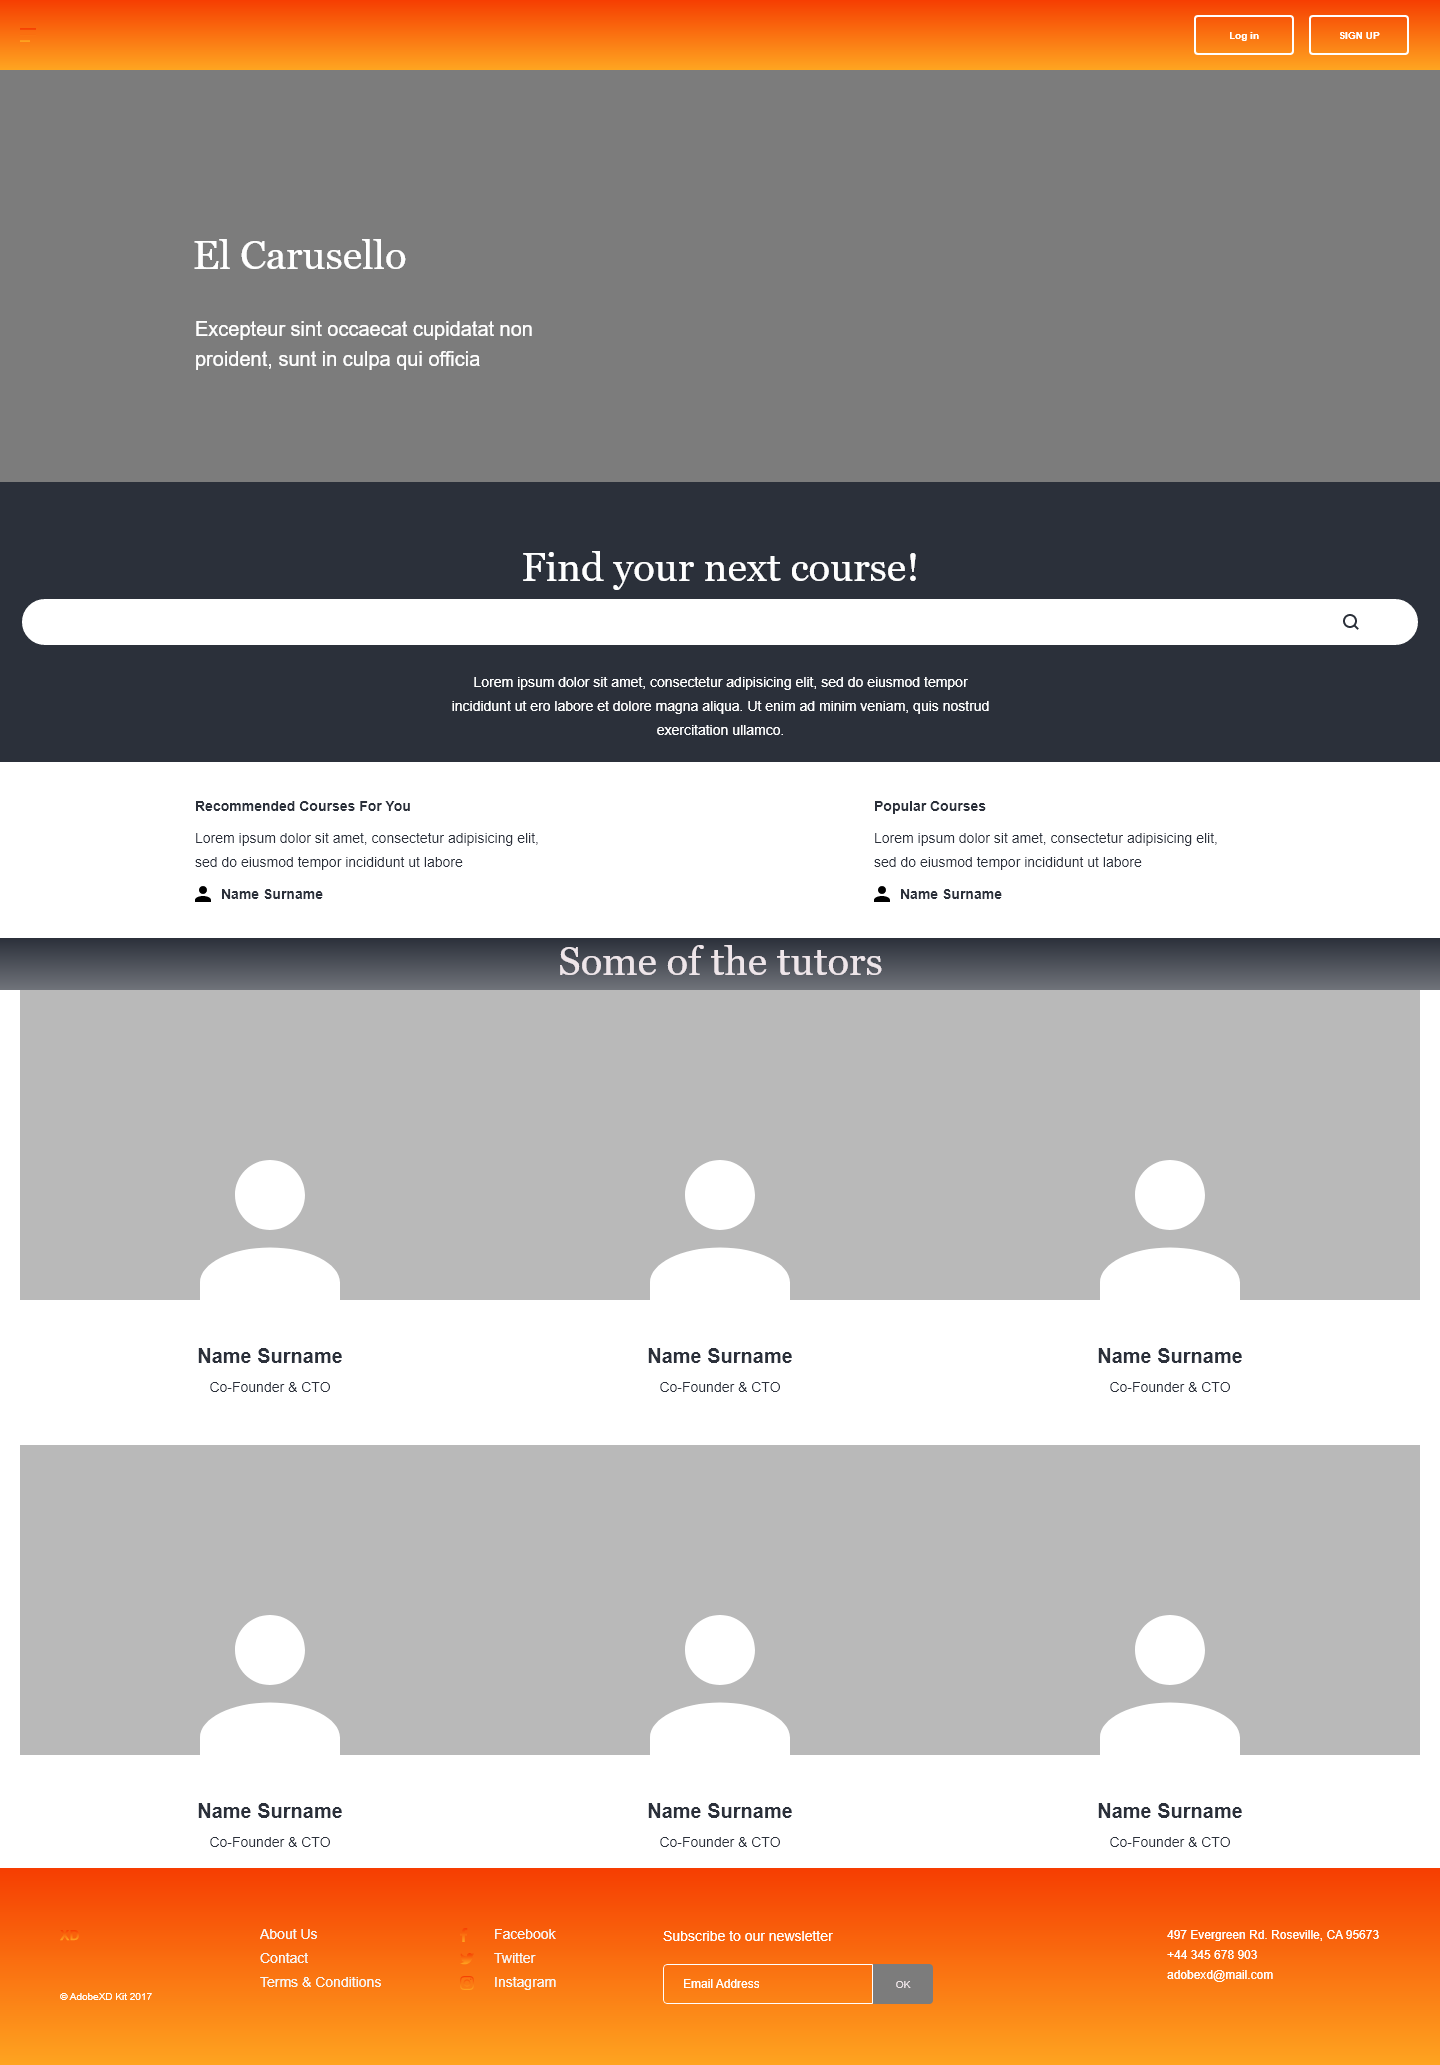
\includegraphics[scale=0.25]{/prototypes/landing-page.png}
    \caption{The landing page for the system}
    \label{fig:landing-page}
\end{figure}
\noindent
\\\\
\autoref{fig:landing-page} shows the landing page.
It is the first page that the users of the system will see, and thus it is important that this page shows some interesting content. 
This page can be accessed both with and without being logged in. 
We have a top bar that changes depending on if the user is logged in or not. 
At the top of the landing page, we will have a carousel that shows some interesting images.
Underneath, we have included a search functionality to find a course or a specific tutor. 
The user should be able to search for both tutors and courses. 
Finally, there will be some recommendations for the user, which will suggest specific tutors based on their profile information and previously taken courses.
 \begin{figure}[]
    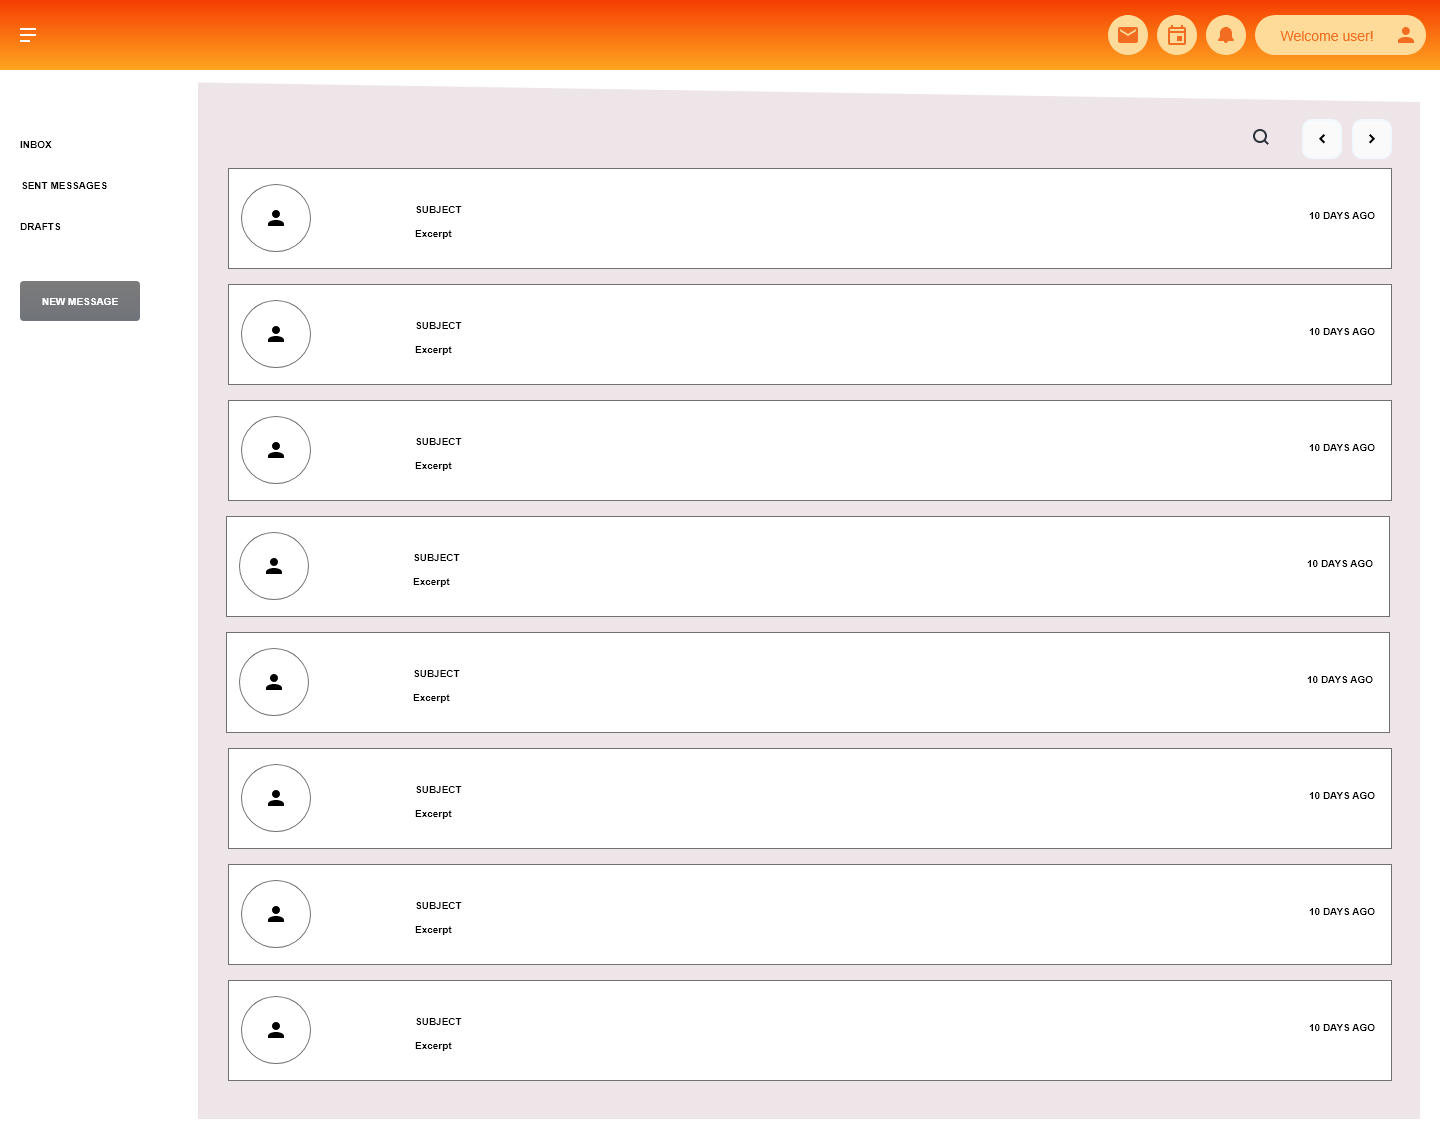
\includegraphics[width=\linewidth]{/prototypes/inbox.png}
     \caption{The inbox for the messaging component in the system}
     \label{fig:inbox}
 \end{figure}
 \noindent
 \\\\
When the user clicks the message icon in the top bar they will be redirected to the inbox page shown on \autoref{fig:inbox}.
Here they can view their recent messages. 
We considered including a search functionality to find specific messages but ultimately did not add it to the prototypes. 
The most recently received messages should be shown on the top of the list, so they are easy to find. 
When a message is received, the topbar should also show a notification for this. 
There should also be an indicator that shows if the user has unread messages. 
The user can click a button on the left side of the page to start writing a new message. 
 \begin{figure}[]
    \centering
    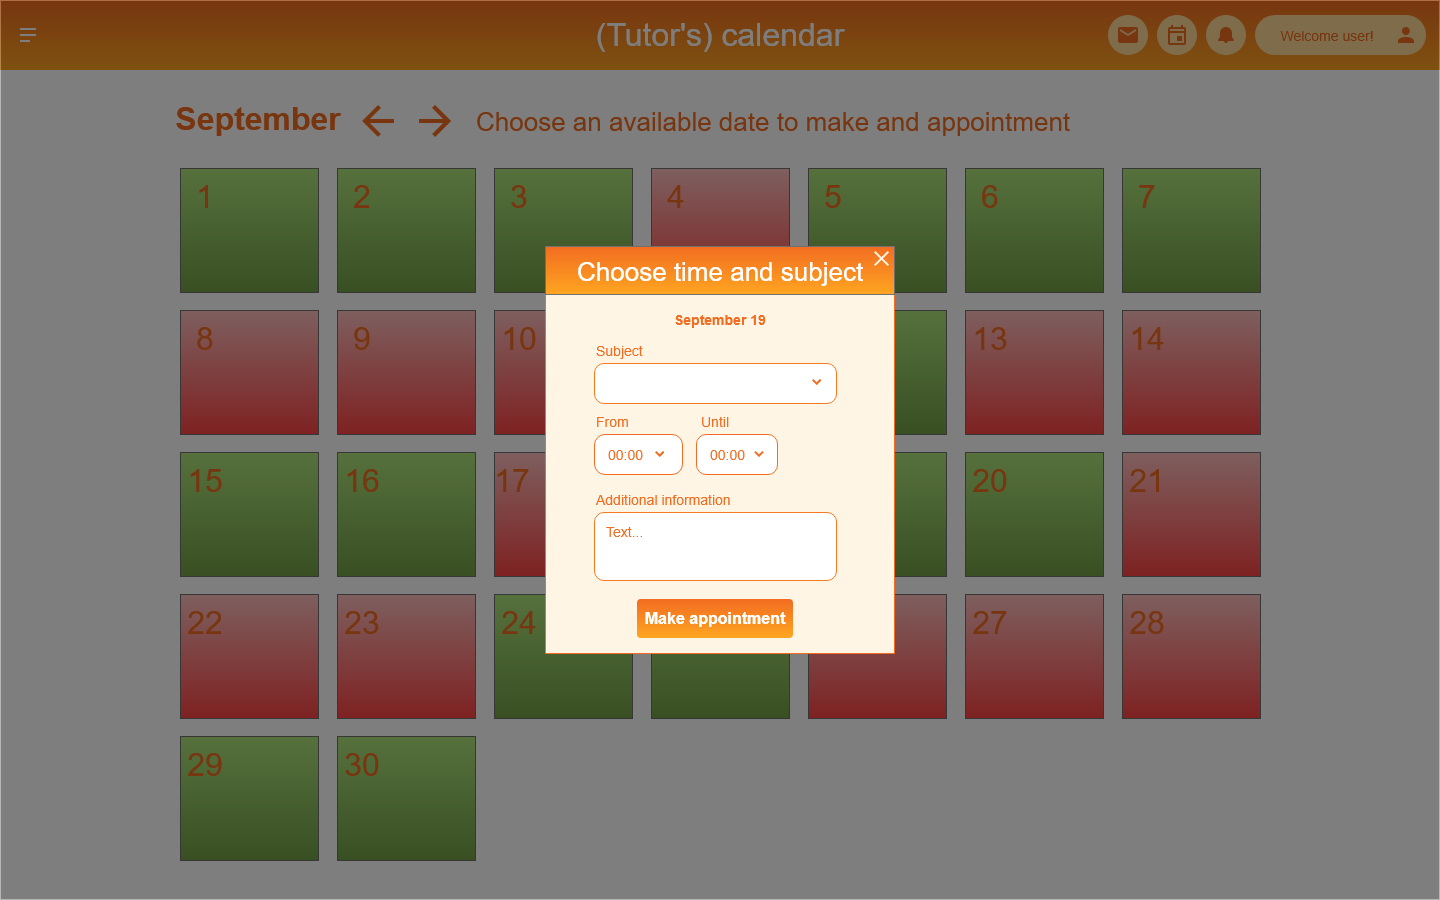
\includegraphics[scale=0.2]{/prototypes/make-appointment.png}
     \caption{Page that shows a tutor's calendar where the student can request an appointment}
     \label{fig:make-appointment}
 \end{figure}
 \noindent
\\\\
 \autoref{fig:make-appointment} is the tutor's calendar from a student's point of view. 
 The student is able to browse the tutor's calendar and look for a date where the tutor is available, shown as the color green. 
 The student then clicks the desired date, and the popup window will show. 
 Here they can specify the subject they wish to be taught and the timeslot as well as additional information. 
 They can only choose one of the tutors available subjects, and the timeslot should comply with the tutor's availability. 
 The tutor also needs to choose what time they are available prior to this.
 When the student makes the appointment, they will be sent to a payment page, and a request will be sent to the tutor, which they can either accept or deny.
 However, the money will not be withdrawn from the student's account until the tutor has approved the appointment.
 \begin{figure}[]
    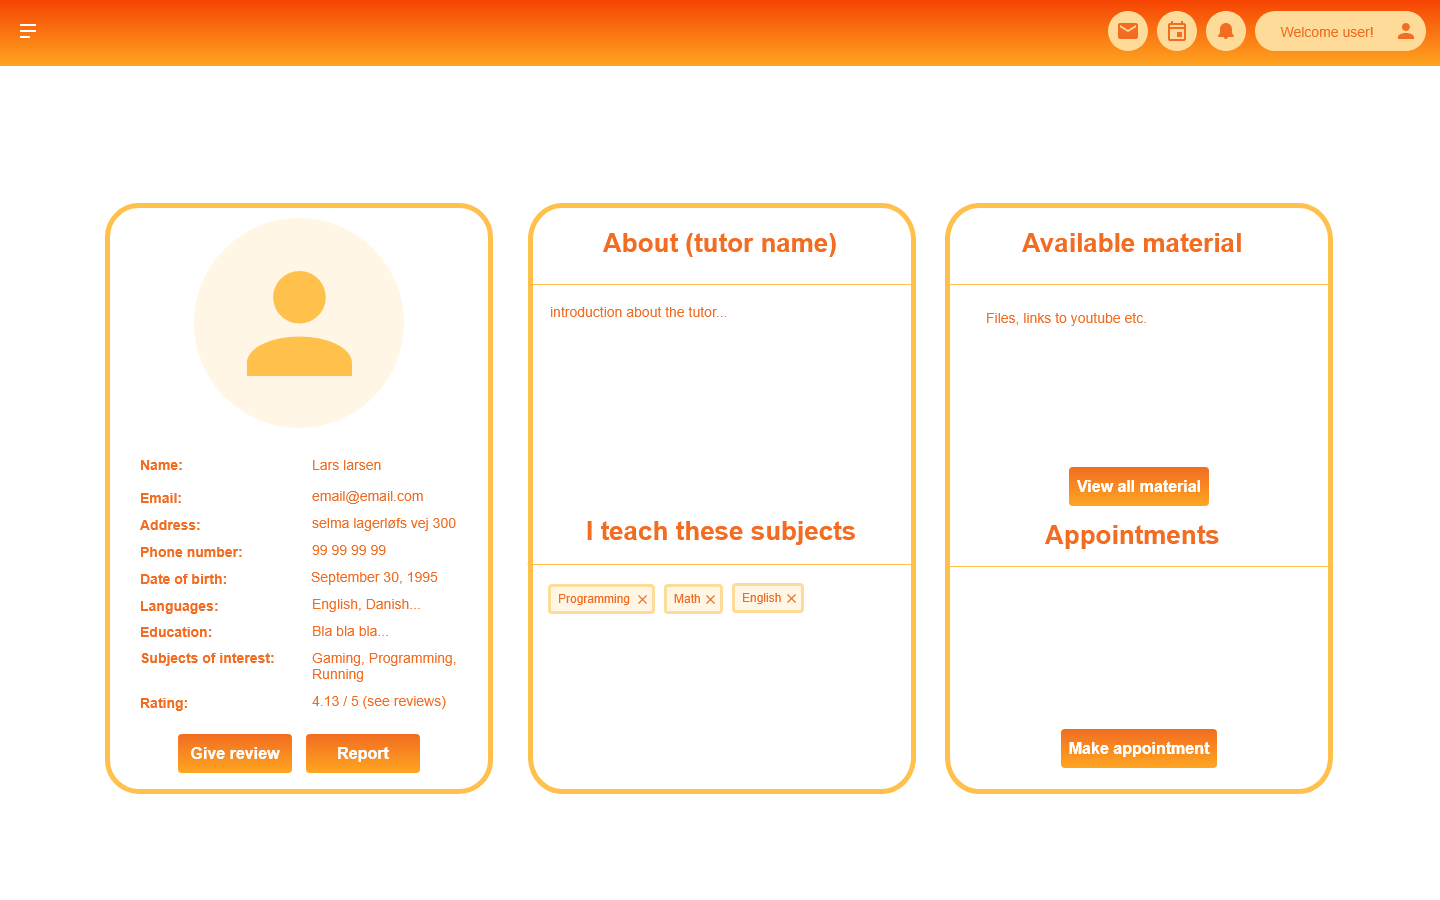
\includegraphics[scale=0.25]{/prototypes/view-information-on-tutor.png}
     \caption{The page where other users can view information about a specific tutor}
     \label{fig:view-information-on-tutor}
 \end{figure}
 \noindent
 \\\\
The page where other users can go and view information about another tutor is shown on \autoref{fig:view-information-on-tutor}. 
Much information should be available here so that a user can know if this tutor can be helpful to them.
The page will show basic information on the left side and also show the tutor's rating. 
A user can click \textit{see reviews} to see what other users wrote about the tutor. 
The user viewing the tutor's page can also leave a review of the tutor or report the tutor if they had a bad experience. 
The tutor can display some written information about them in the middle that others can read. 
The middle also shows which subjects the tutor teaches. 
A tutor also has some material connected to their page if they have uploaded any. 
They can make this available to others however they wish, but can also lock it behind payment or only make it available if a student books an appointment with the tutor.
Users can click the \textit{View all material} button to go to the view material page where all the files and links can be found. 
Finally, the user can wish to make an appointment with the tutor. 
By clicking the \textit{Make appointment} button, the user is redirected to the tutor's calendar, where they can find a suitable date for the appointment. 
 \begin{figure}[]
    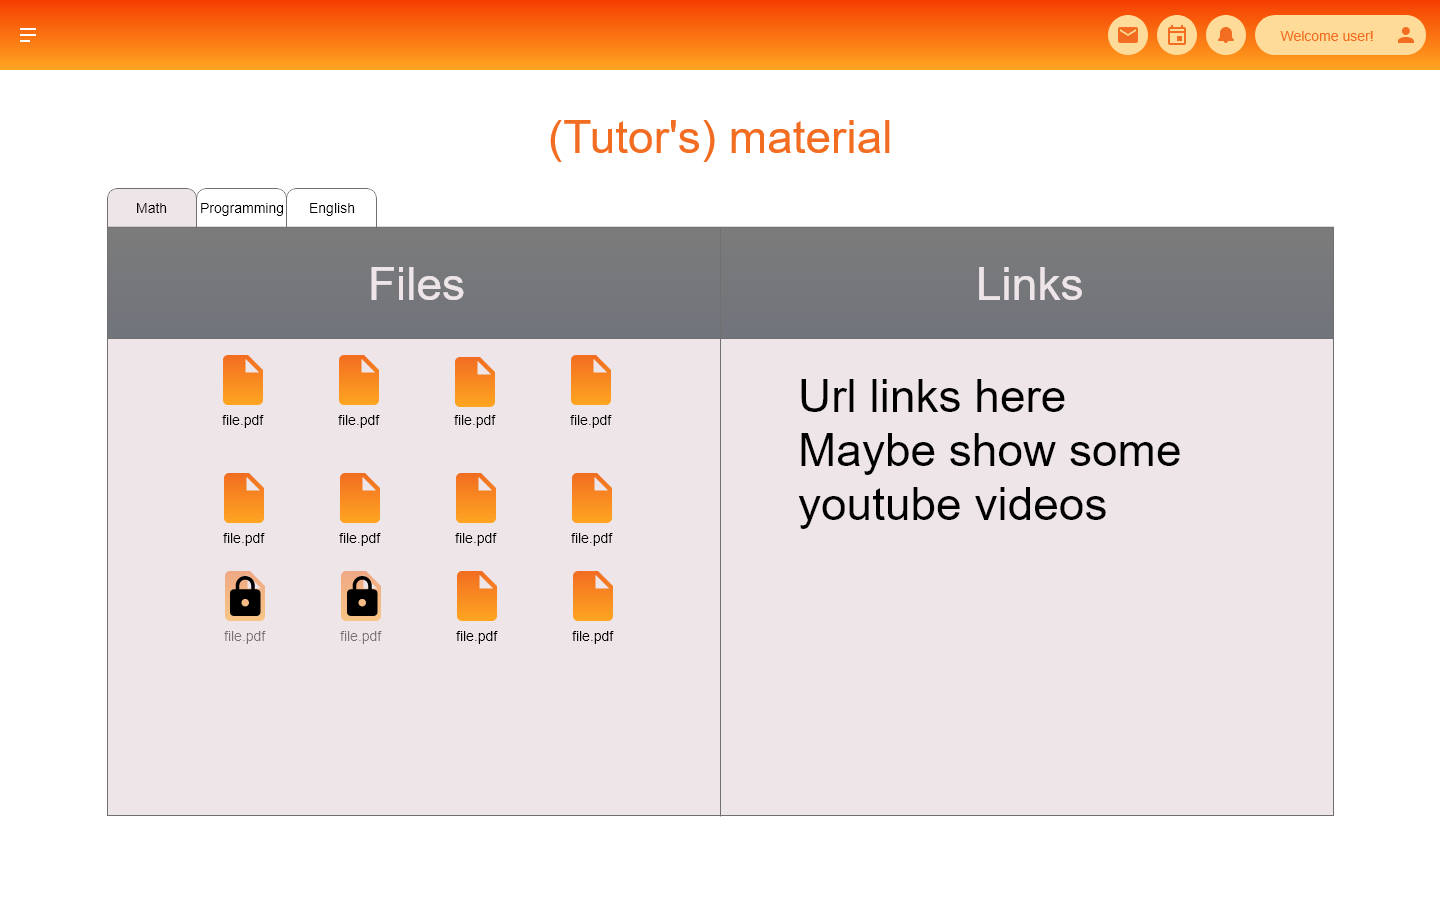
\includegraphics[width=\linewidth]{/prototypes/view-tutor-material.png}
     \caption{The page that shows a tutors available material}
     \label{fig:view-tutor-material}
 \end{figure}
 \noindent
 \\\\
\autoref{fig:view-tutor-material} shows a specific tutor's uploaded material. 
The material is divided into which subject it belongs to make it easier for other users to find the relevant material. 
The material can be any kind of file, or it can be links to useful pages such as some reading material or perhaps a YouTube video. 
When a specific user goes to a tutor's material page, only the material that is accessible to them should be made available. 
All other files should show a lock on top of the file or link to indicate that this item is not available. 
The user can then hover over this item, and it should then tell the user how it can be unlocked. 
